\section{Stand der Technik}\ref{StandDerTechnik}
\subsection{MyPost 24}
\subsubsection{Allgemein}
Mit der Pick Post und My Post 24 können Briefe und Pakete an die genannte Pick-Up Station gesendet werden. Es besteht auch das Angebot, Pakete von einer Pick-Up Station zu versenden. 
Die Auswahl einer Pick-Up Station geschieht dabei mit der Angabe der entsprechenden Station. Der Dienst lässt sich somit in jedem Onlineshop nutzen.\\
Die Abholung der Artikel muss innerhalb von 10 Tagen geschehen. Sobald die Artikel zur Abholung bereit sind, erhält der Kunde wahlweise eine Bestätigungsmail oder ein SMS. Mit dem darin enthaltenen Abholcode lässt sich die Ware abholen. 
[\cite{postPickUp}]\\
Im Grossraum Luzern befinden sich acht My Post 24-Abholstellen. [\cite{myPost24Stations}]
Das Design der Abholstelle sieht dabei konventionellen Briefkästen der Post sehr ähnlich. 
\begin{figure}[H]
	\centering
	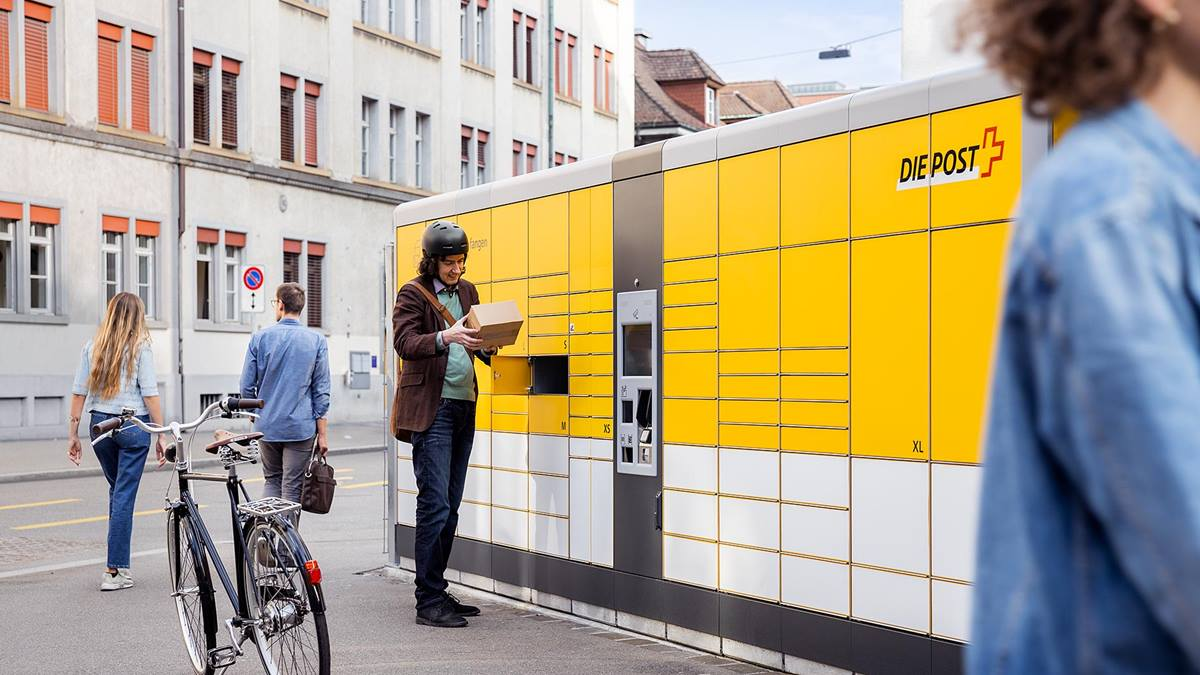
\includegraphics[width=1\textwidth]{images/myPostImage.jpg}
	\caption[My Post 24-Abholstelle]{My Post 24-Abholstelle,\\ Quelle: \cite{myPost24StationsImage}}
	\label{img: My Post 24-Abholstelle}
\end{figure}
Die Lösung der Post behebt dabei aber nicht die in Kapitel \ref{Problem} beschriebenen Probleme. Das Angebot richtet sich hauptsächlich an Personen, welche bei der Lieferung der Post nicht zuhause sind. Durch das Angebot kann so ein Abholen an der Poststelle vermieden werden. Die Lieferzeit sowie die Lieferkosten bleiben dabei aber vorhanden. Der Bestell- und Bezahlvorgang wird beim jeweiligen Onlineshop durchgeführt. 
\newpage 
\subsection{avec}
\subsubsection{avec now}
" — Dein Online Lieferservice von avec —
 Mit avec now haben wir rund um das beliebte Angebot unseres Convenience-Formats avec einen Online-Store lanciert.
 Zur Auswahl steht ein breites Convenience-Sortiment. Die bestellten Waren werden direkt in unseren Stores zusammengestellt und so schnell wie möglich ausgeliefert."[\cite{avecNow}]
 
 Auf der Website von avec now wird dabei eine Lieferzeit von 60 Minuten angepriesen. Der Mindestbestellwert beträgt dabei 20.- Fr.[\cite{avecNowMain}]
 Das Angebot gilt dabei für einen grossen Teil des Sortiments, darunter auch Tabakwaren. Das Angebot befindet sich dabei noch in der Pilotphase und wird nur im Raum Zürich angeboten. [\cite{avecNowShipping}]
 
 \subsubsection{avec Box}\label{avecBox}
 Der Anbieter geht bei diesem Angebot einen neuen Weg. Das gesamte Einkaufen wird mittels App durchgeführt. Mittels dieser können Produkte dem Warenkorb hinzugefügt und so bezogen werden. In einer ersten Phase sind zu Stosszeiten Mitarbeiter präsent, um die Kunden beim Einkauf zu unterstützen.  \\
 Um Tabakprodukte zu beziehen, befindet sich in der App eine integrierte Altersverifikation. Die Tabakwaren werden dabei im Store via Touchscreen ausgewählt. Durch die App wird eine Altersverifikation durchgeführt. [\cite{avecBoxTabak}]
 \begin{figure}[H]
 	\centering
 	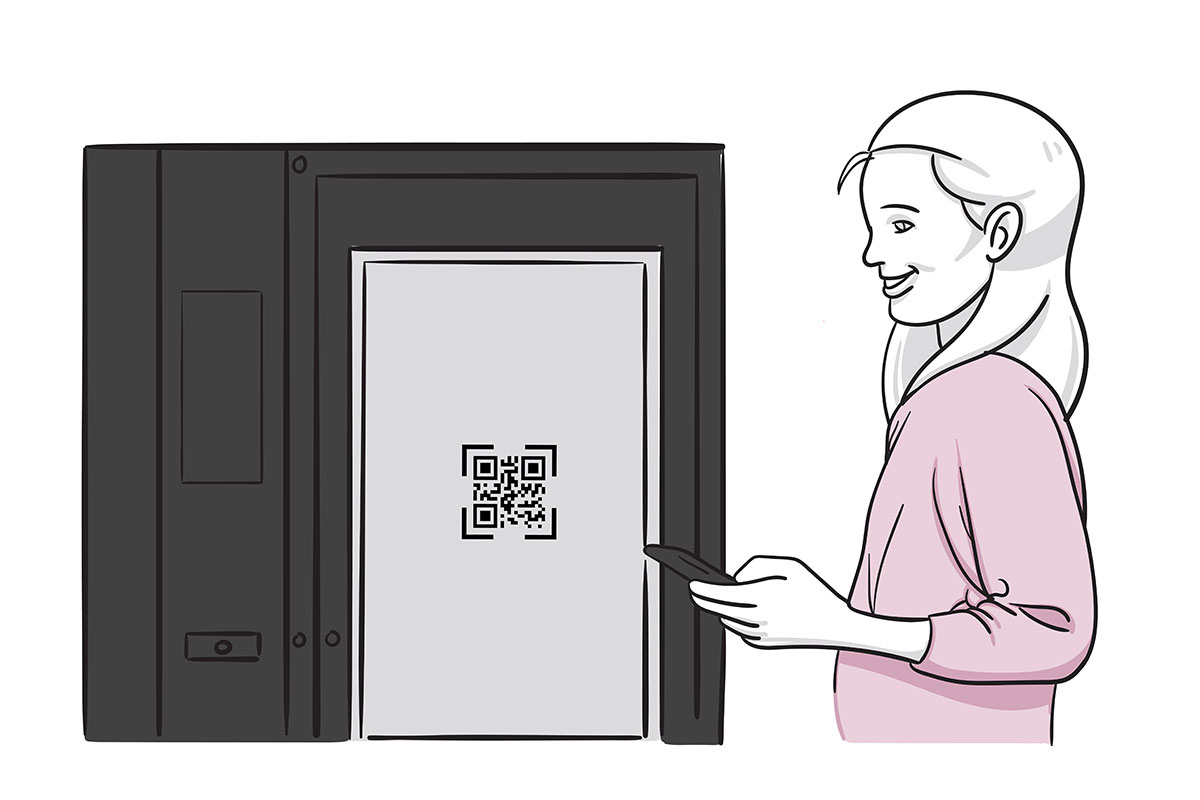
\includegraphics[width=1\textwidth]{images/tabakkaufAvecBox.jpg}
 	\caption[Tabakkauf avec box]{Tabakkauf avec box,\\ Quelle: \cite{avecBoxTabak}}
 	\label{img: avec box tabakkauf}
 \end{figure}
 
 Nach momentanem Stand steht die avec box am Campus der ETH Zürich. Die Box ist dabei von Montag-Sonntag jeweils von 6:00 - 22:00 in Betrieb. Es ist ein Rollout in weitere Regionen der Schweiz vorgesehen. [\cite{avecBoxStand}]\\
 Das Angebot von avec löst einige der genannten Probleme. So kann die Ware direkt bezogen werden. Es fallen keine Versandkosten an. Zur Zeit ist die avec box nur an einem Standort verfügbar, was die Verfügbarkeit erheblich einschränkt. Zudem ist sie nur zwischen 6:00-22:00 in Betrieb. 
 
 \subsubsection{Ablauf Tabakkauf}
Die avec box ist sehr ähnlich zur JTI Pick-Up Station. Aus diesem Grund wird der Registrierungsvorgang nachfolgend genauer betrachtet. 
\paragraph{Registrierung}
Das Anlegen eines avec-Kontos verläuft dabei analog zur Erstellung von anderen Accounts. Mittels Handynummer und Passwort wird der Account angelegt. Zur Verifikation wird ein Bestätigungscode an die Nummer gesendet. Dieser muss eingegeben werden. Anschliessend wird die Alterverifikation durchgeführt. Hierzu muss die Identitätskarte mit der Kamera eingelesen werden. In einem nächsten Schritt kann die Kreditkarte hinterlegt werden. Der Bezahldienst wird dabei von Datatrans bereitgestellt. Anschliessend ist die Registierung abgeschlossen und der Einkauf in der avec box könnte beginnen. \\

\begin{figure}[h]
	\begin{subfigure}[b]{0.4\textwidth}
		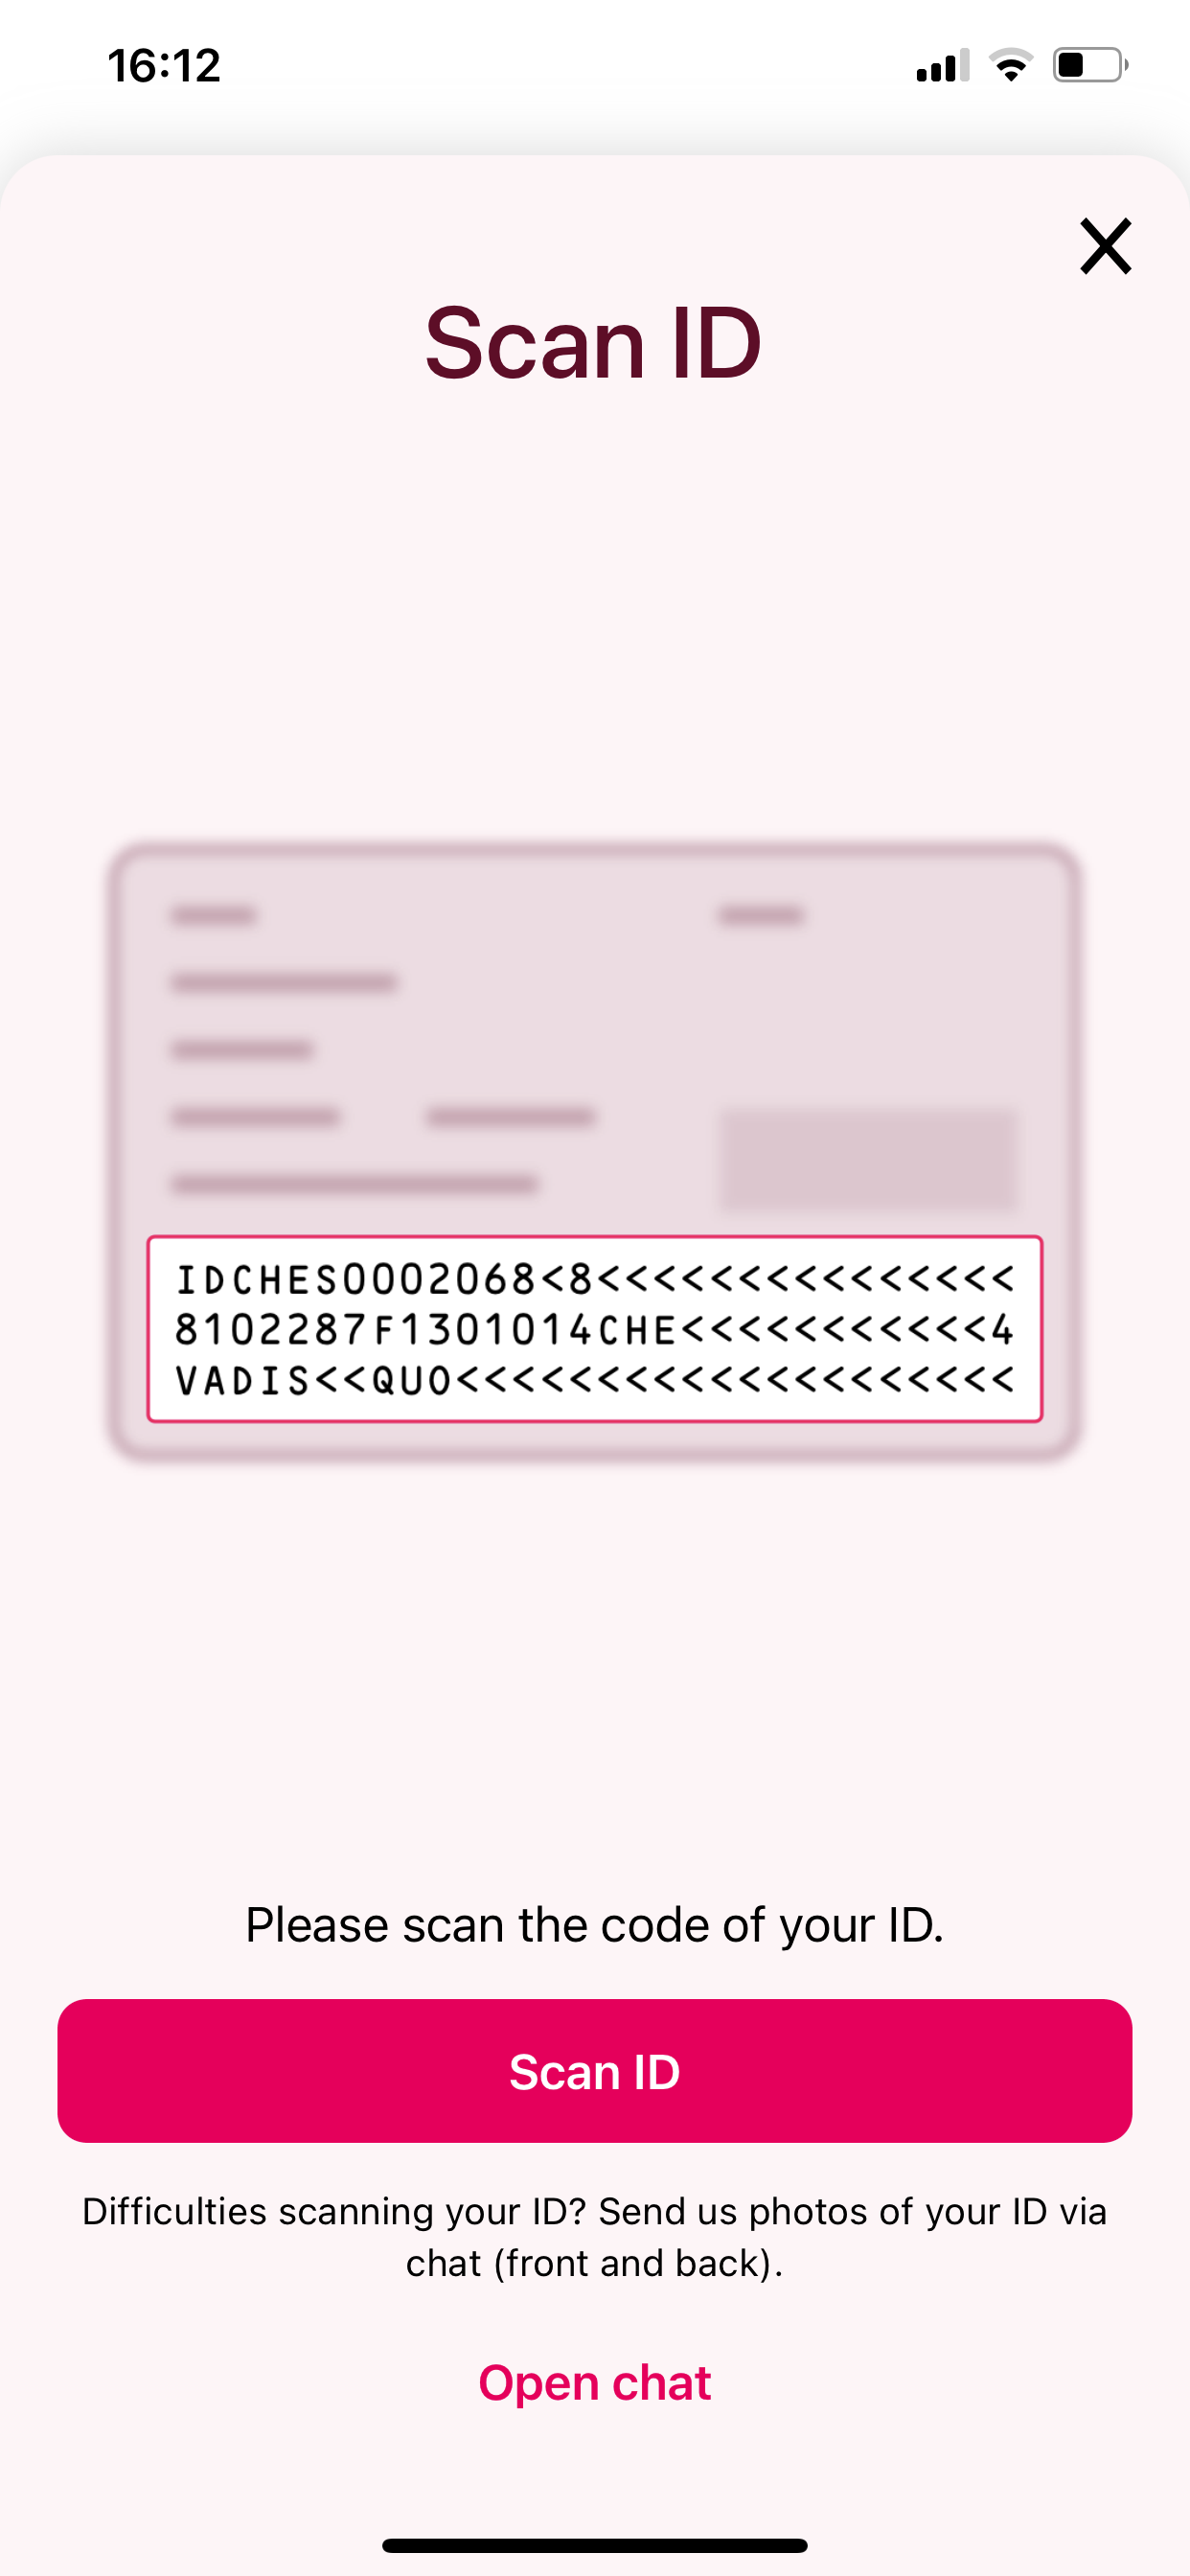
\includegraphics[scale=0.15]{images/ID-Scan.PNG}
		\caption[Einlesen der Identitätskarte]{Einlesen der Identitätskarte,\\ Quelle: \cite{avecApp}}
		\label{img: Einlesen der Identitaetskarte}
	\end{subfigure}
	\hfill
	 \begin{subfigure}[b]{0.4\textwidth}
		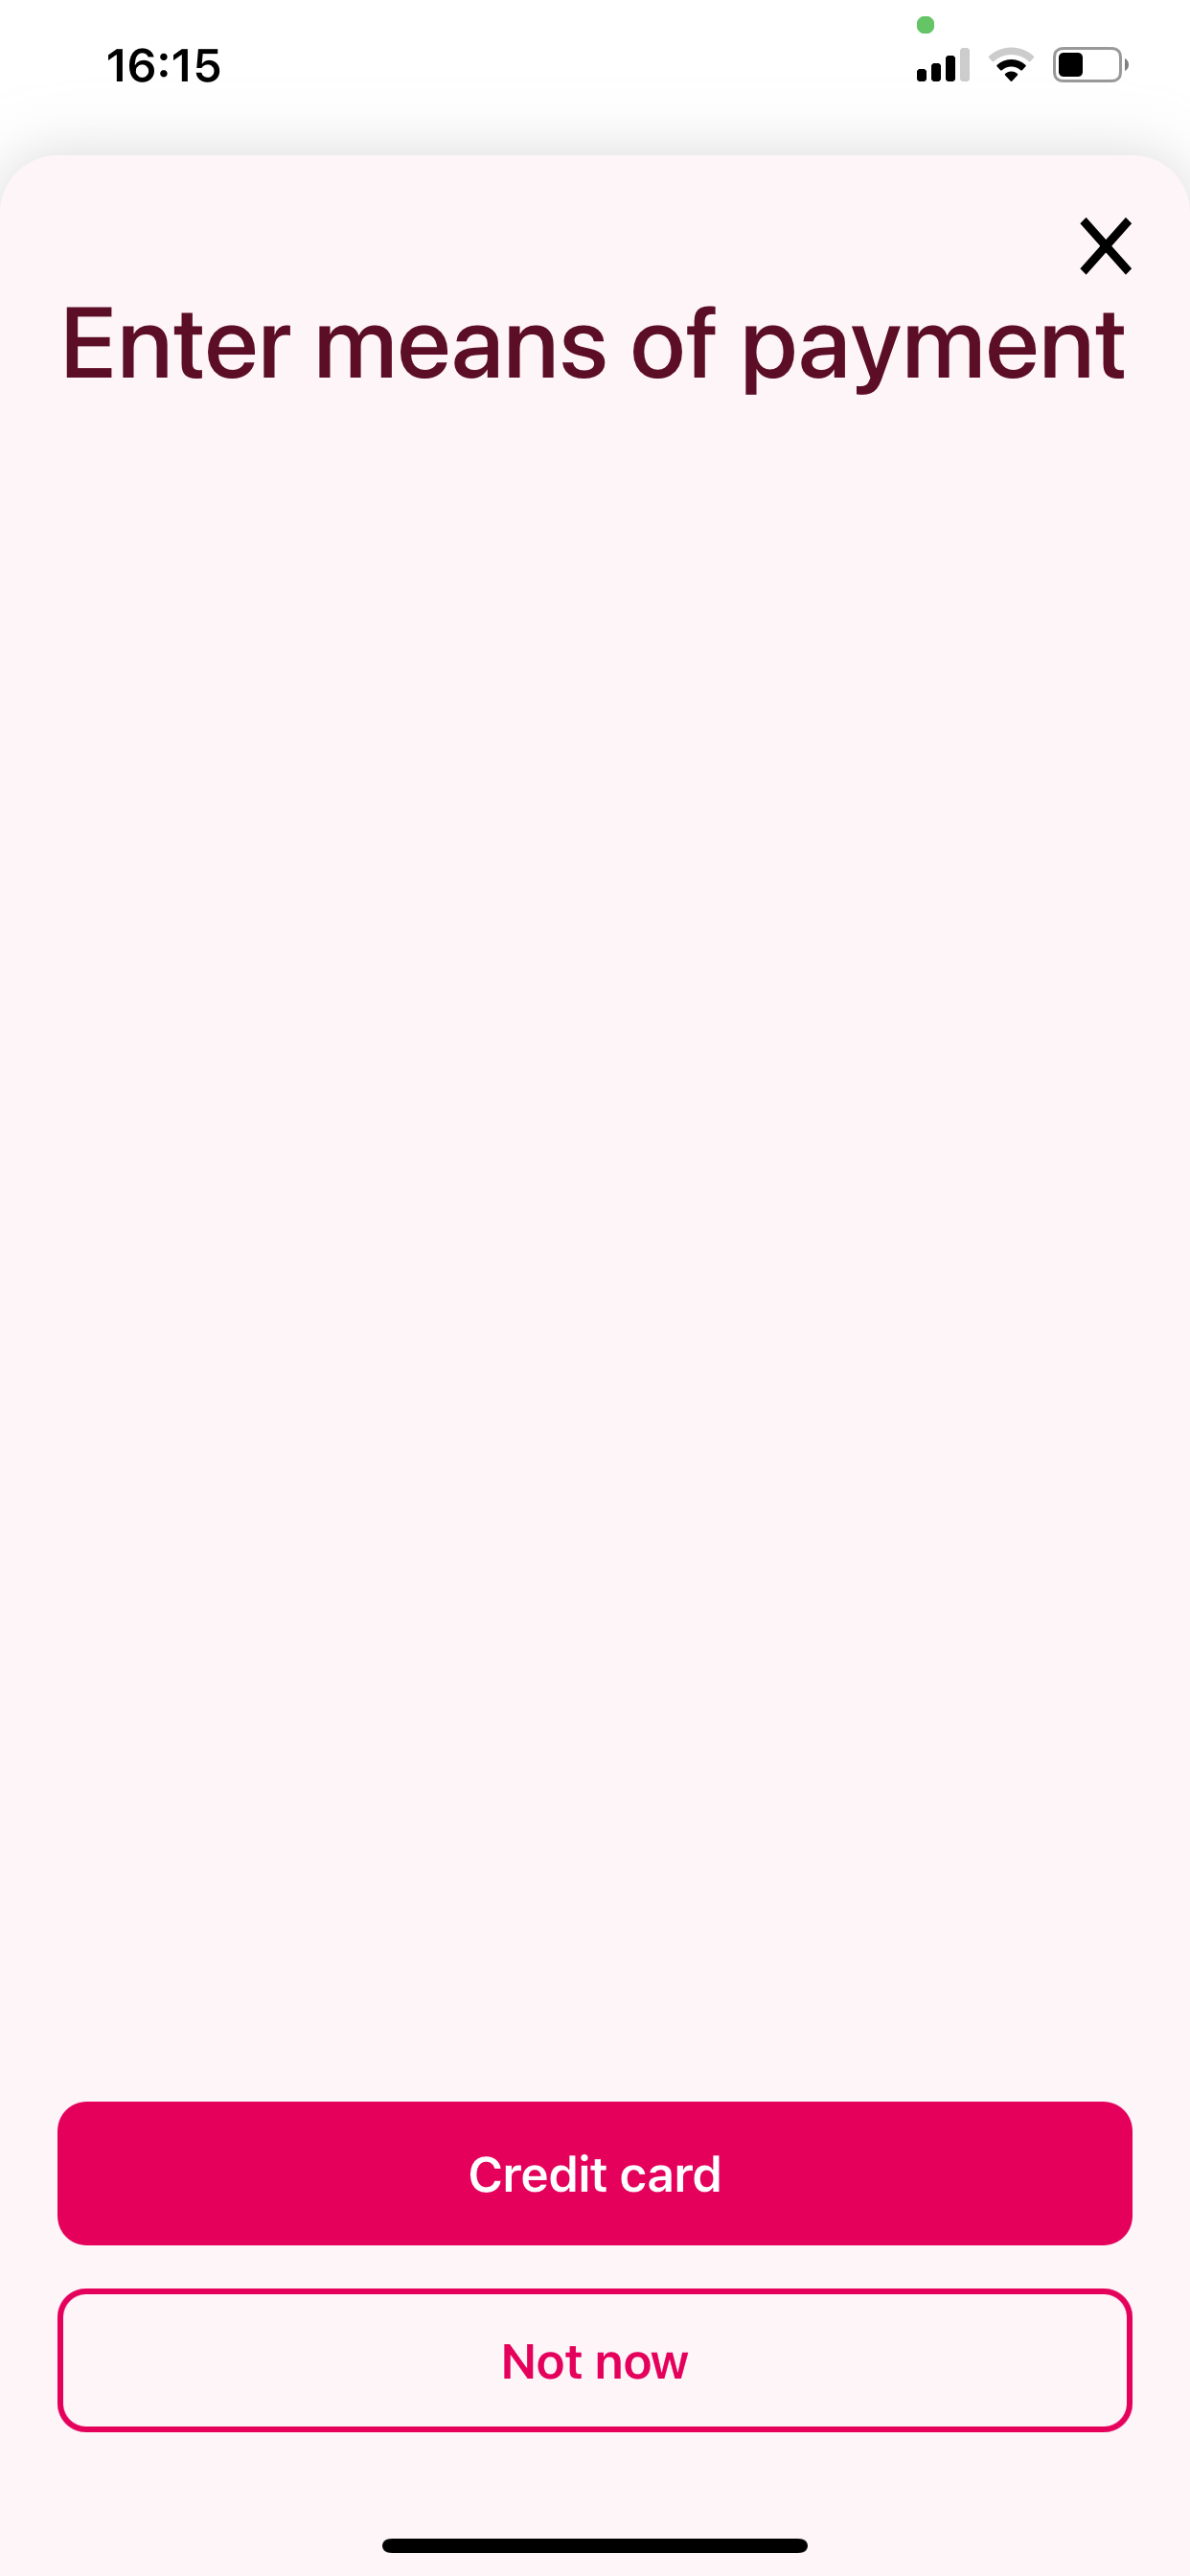
\includegraphics[scale=0.15]{images/creditCard.PNG}
		\caption[Einlesen der Kreditkarte in der avec App]{Einlesen der Kreditkarte in der avec App,\\ Quelle: \cite{avecApp}}
		\label{img: Einlesen der Kreditkarte in der avec App}
	\end{subfigure}
\end{figure}

Leider wird in der Applikation keine Auskunft über den Anbieter der Alterverifikation gegeben. Das Vorgehen ist dabei sehr intuitiv und schnell. 

\subsection{Starbucks \ac{PWA}}
In diversen Quellen wird die \ac{PWA} von Starbucks immer als eine der besten \ac{PWA}'s genannt. [\cite{}] Die Applikation ermöglicht es dem Nutzer, die angebotenen Produkte zu bestellen und diese anschliessend im Store abzuholen. Der Anwendungszweck ist somit ähnlich zur JTI-Pick-Up Station. Sie ist dabei sehr nahe an einer nativen App, wodurch dem Benutzer die Bedienung sehr leicht fällt. Die Applikation reagiert sehr schnell, es sind keine Ladezeiten zu bemerken. Zudem ist die \ac{PWA} auch offline nutzbar. Hierbei kommt es zwar zu Einschränkungen in der Nutzung, jedoch lässt sie sich weiterhin bedienen. 
\begin{figure}[h]
	\begin{subfigure}[b]{0.4\textwidth}
		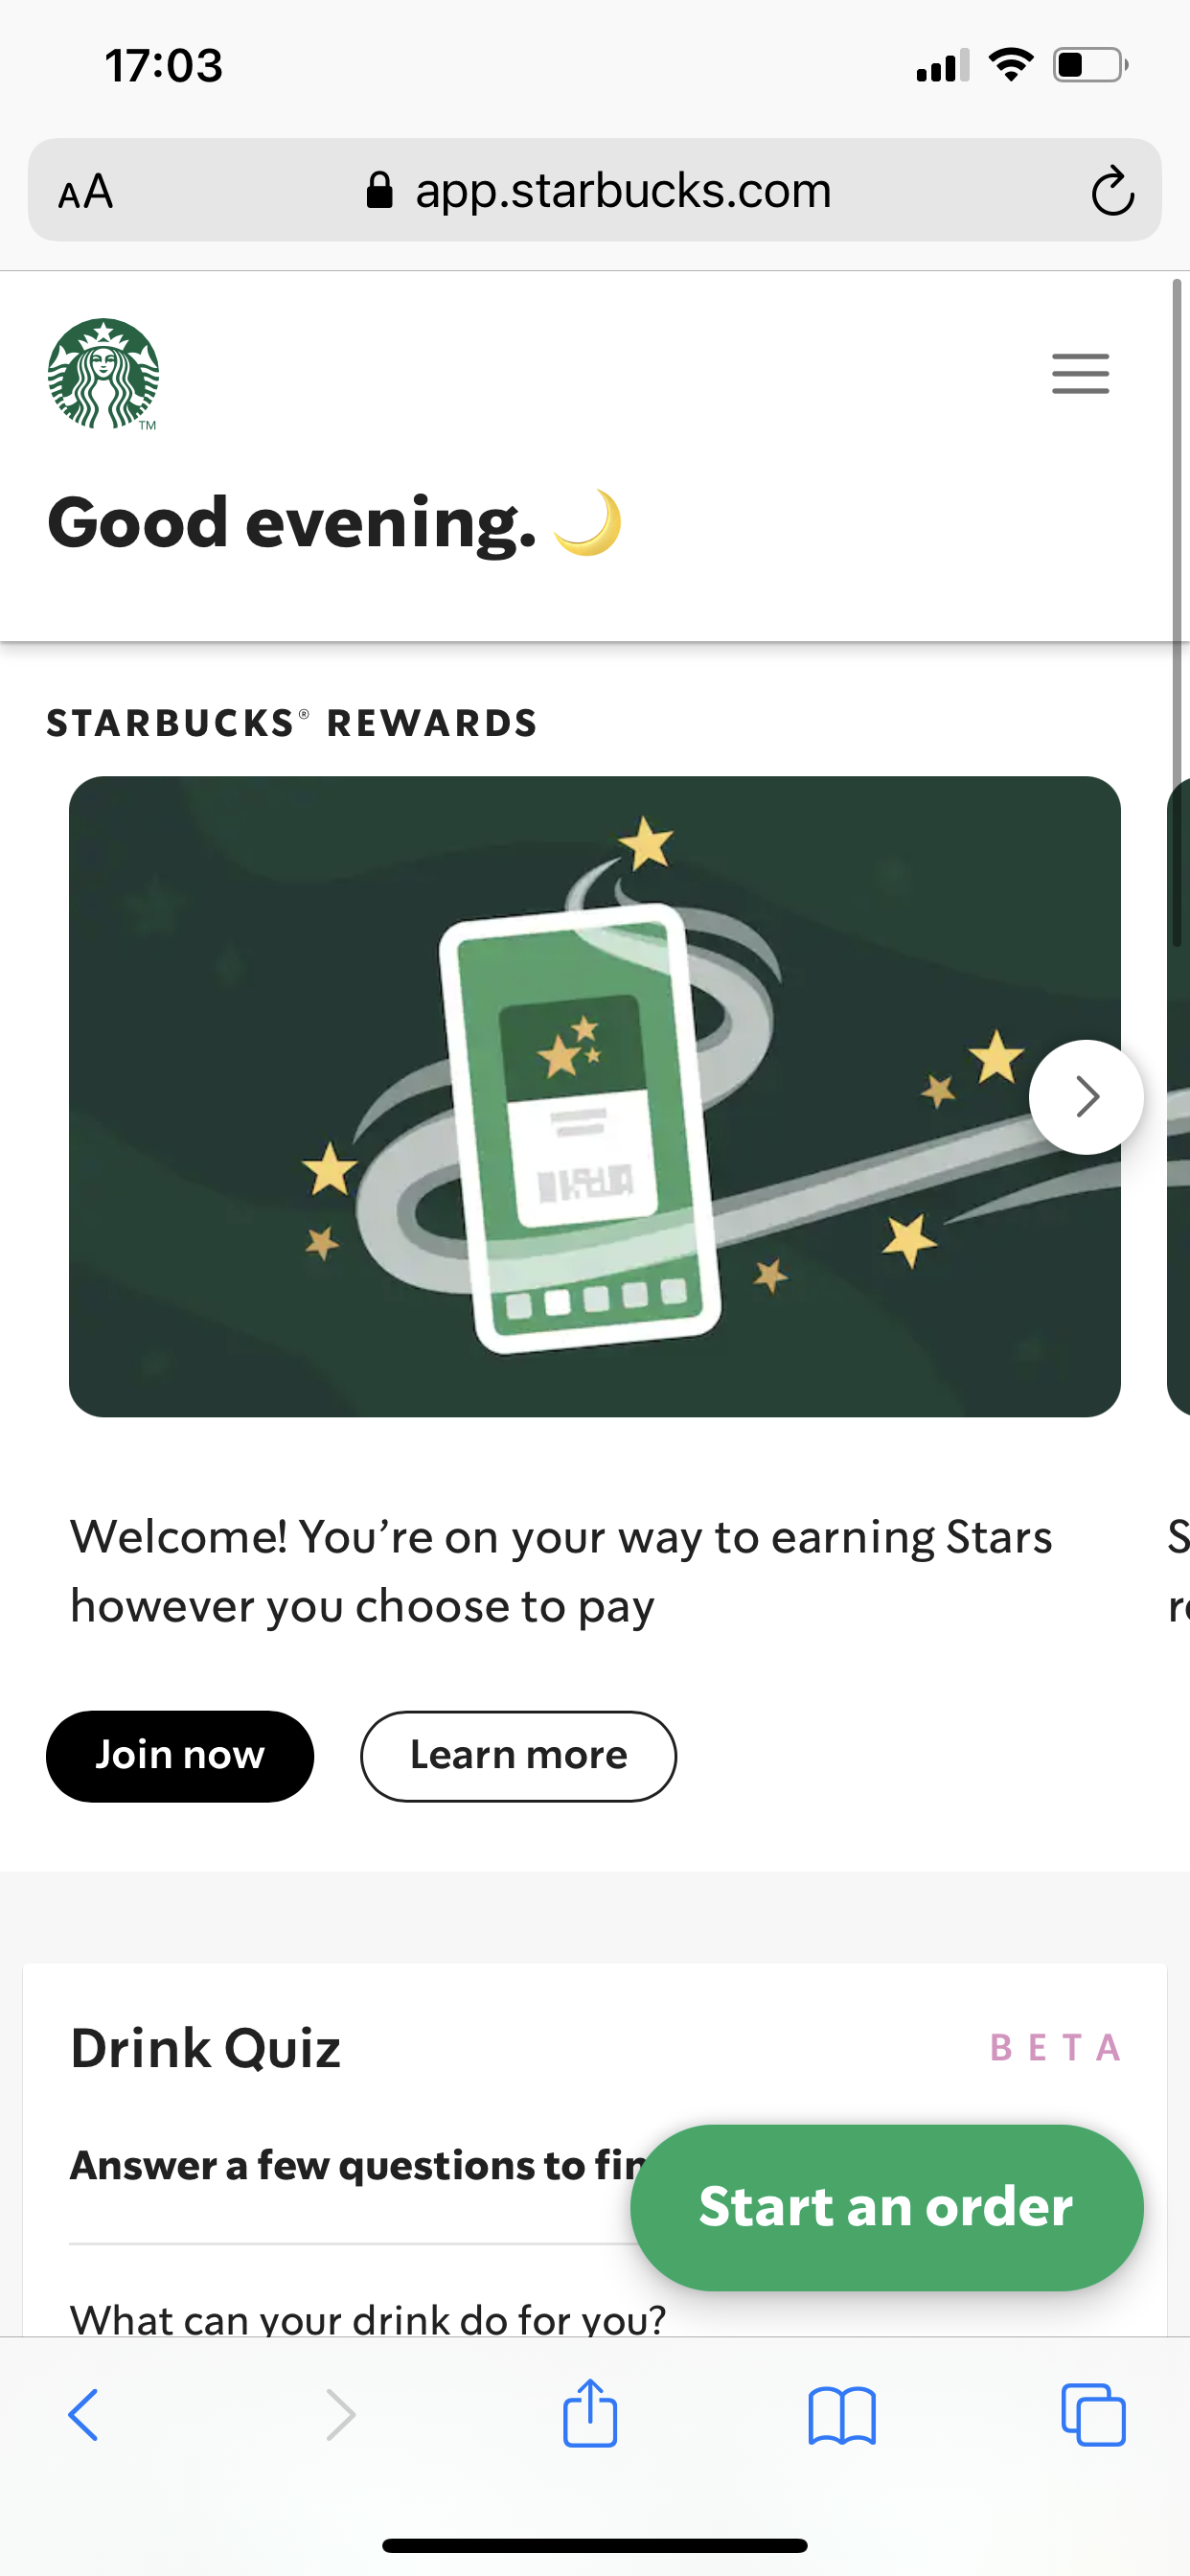
\includegraphics[scale=0.15]{images/starbucks_main.PNG}
		\caption[Startseite der Starbucks \ac{PWA}]{Startseite der Starbucks \ac{PWA},\\ Quelle: \cite{starbucksPwaMain}}
		\label{img: Startseite der Starbucks PWA}
	\end{subfigure}
	\hfill
	\begin{subfigure}[b]{0.4\textwidth}
		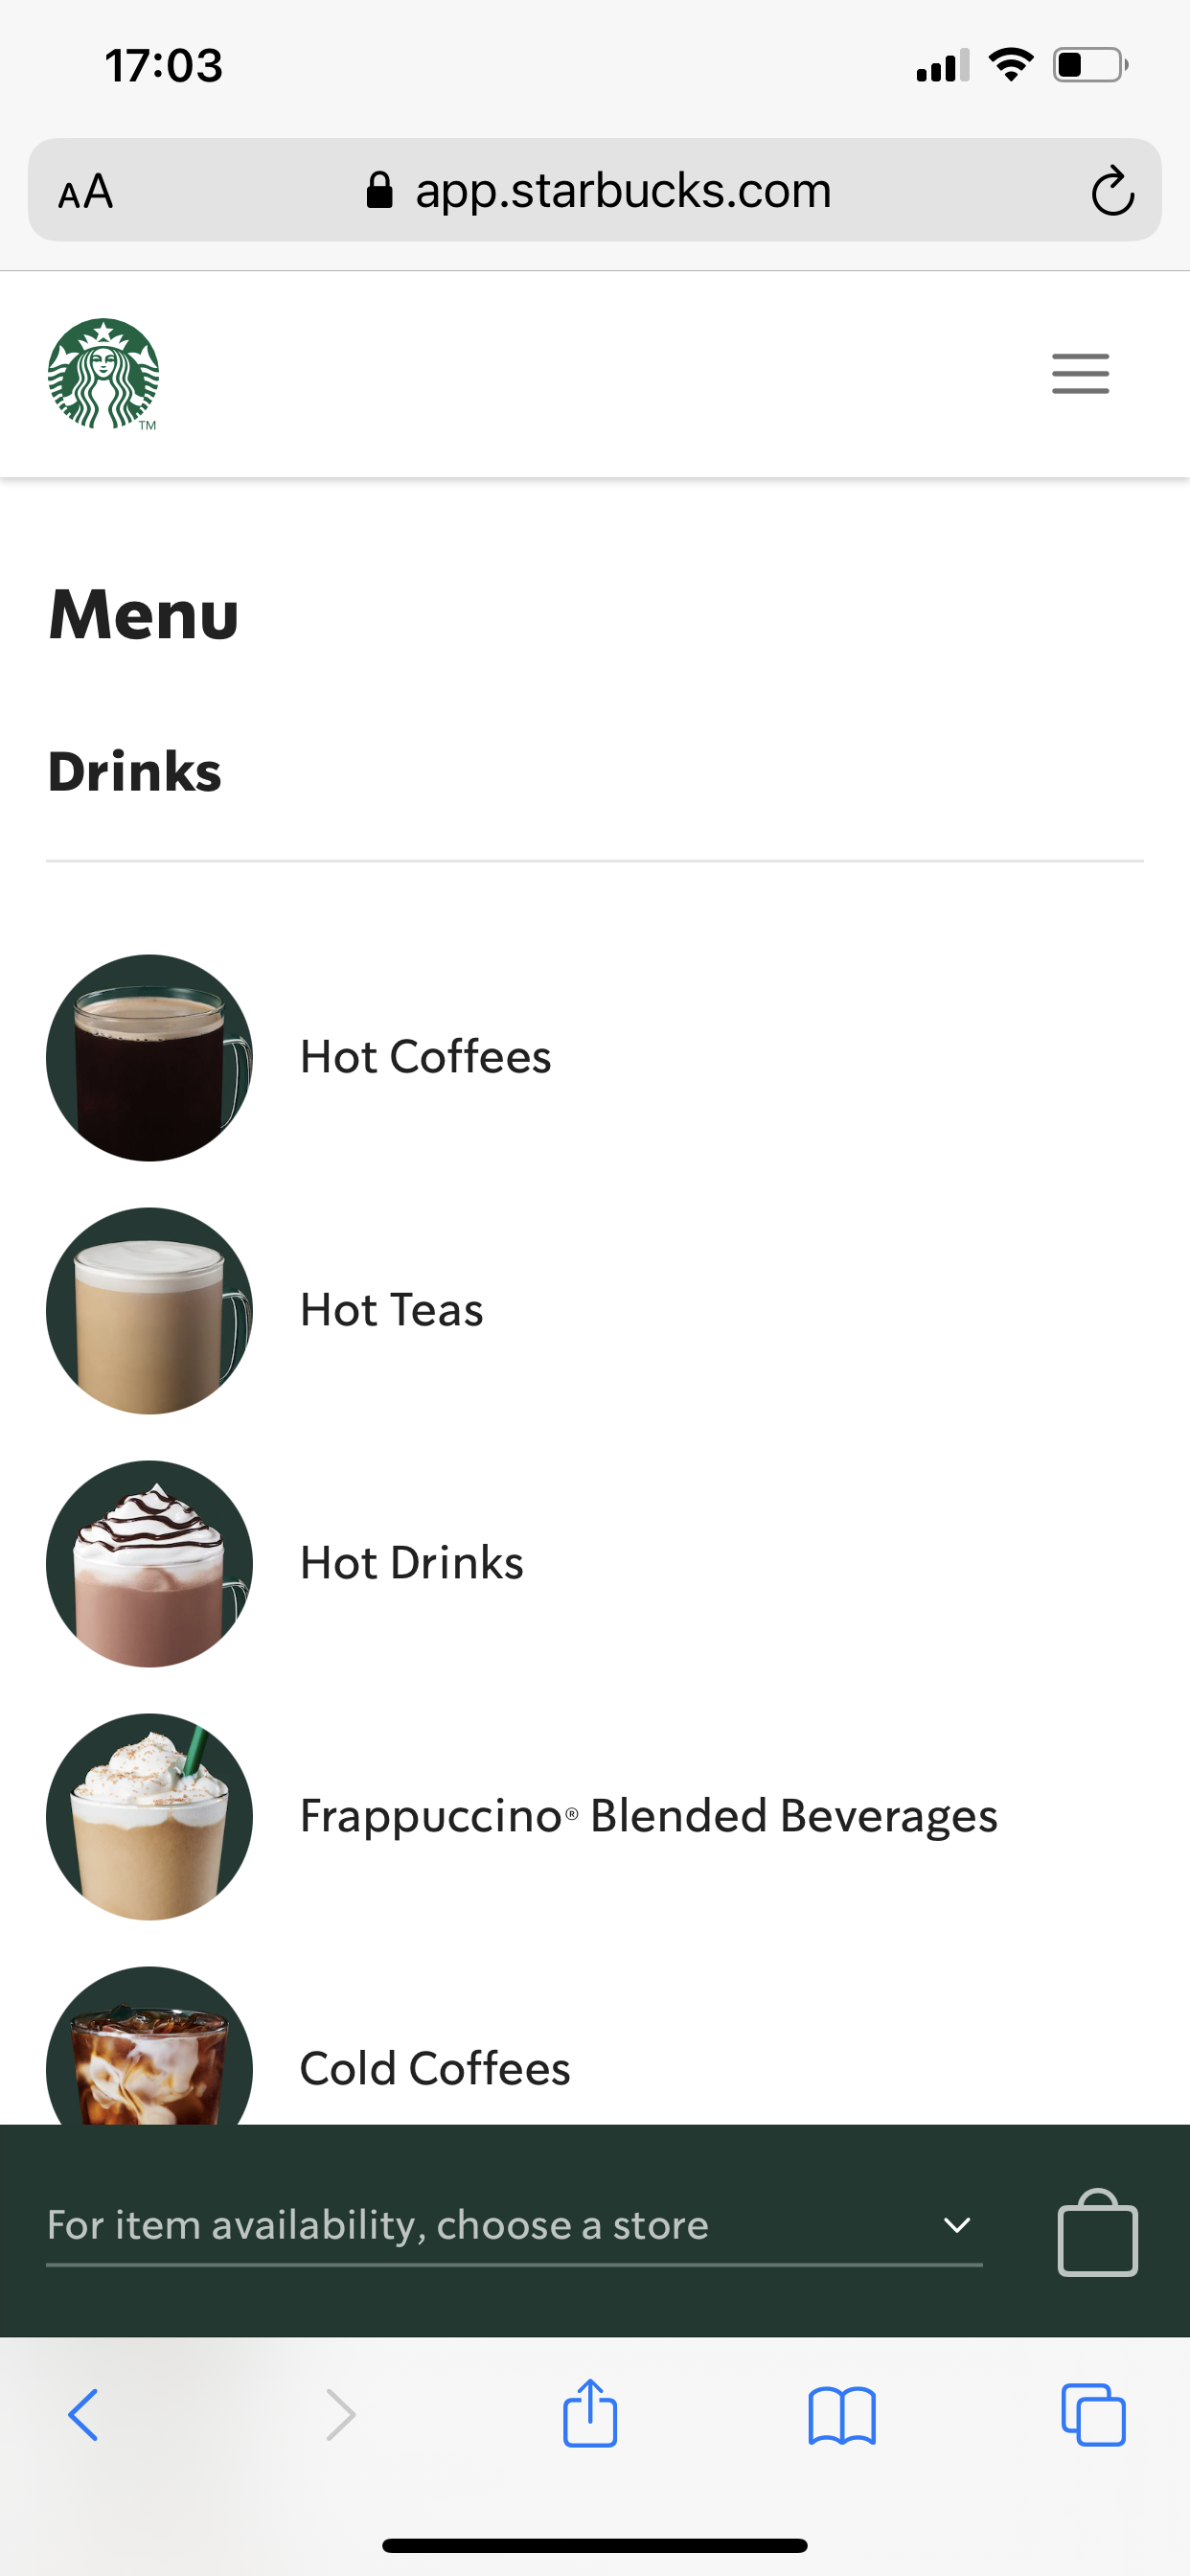
\includegraphics[scale=0.15]{images/starbucks_angebot.PNG}
		\caption[Produktübersicht der Starbucks \ac{PWA}]{Produktübersicht der Starbucks \ac{PWA},\\ Quelle: \cite{starbucksPwaMenu}}
		\label{img: Produktübersicht der Starbucks PWA}
	\end{subfigure}
\end{figure}

\subsubsection{Standortsuche}
Die Applikation bietet auch ein Feature, um die nächstgelegene Starbucksfiliale anzuzeigen. Hierbei wird auf die aktuelle Position des Nutzers zugegriffen. 
 \begin{figure}[H]
	\centering
	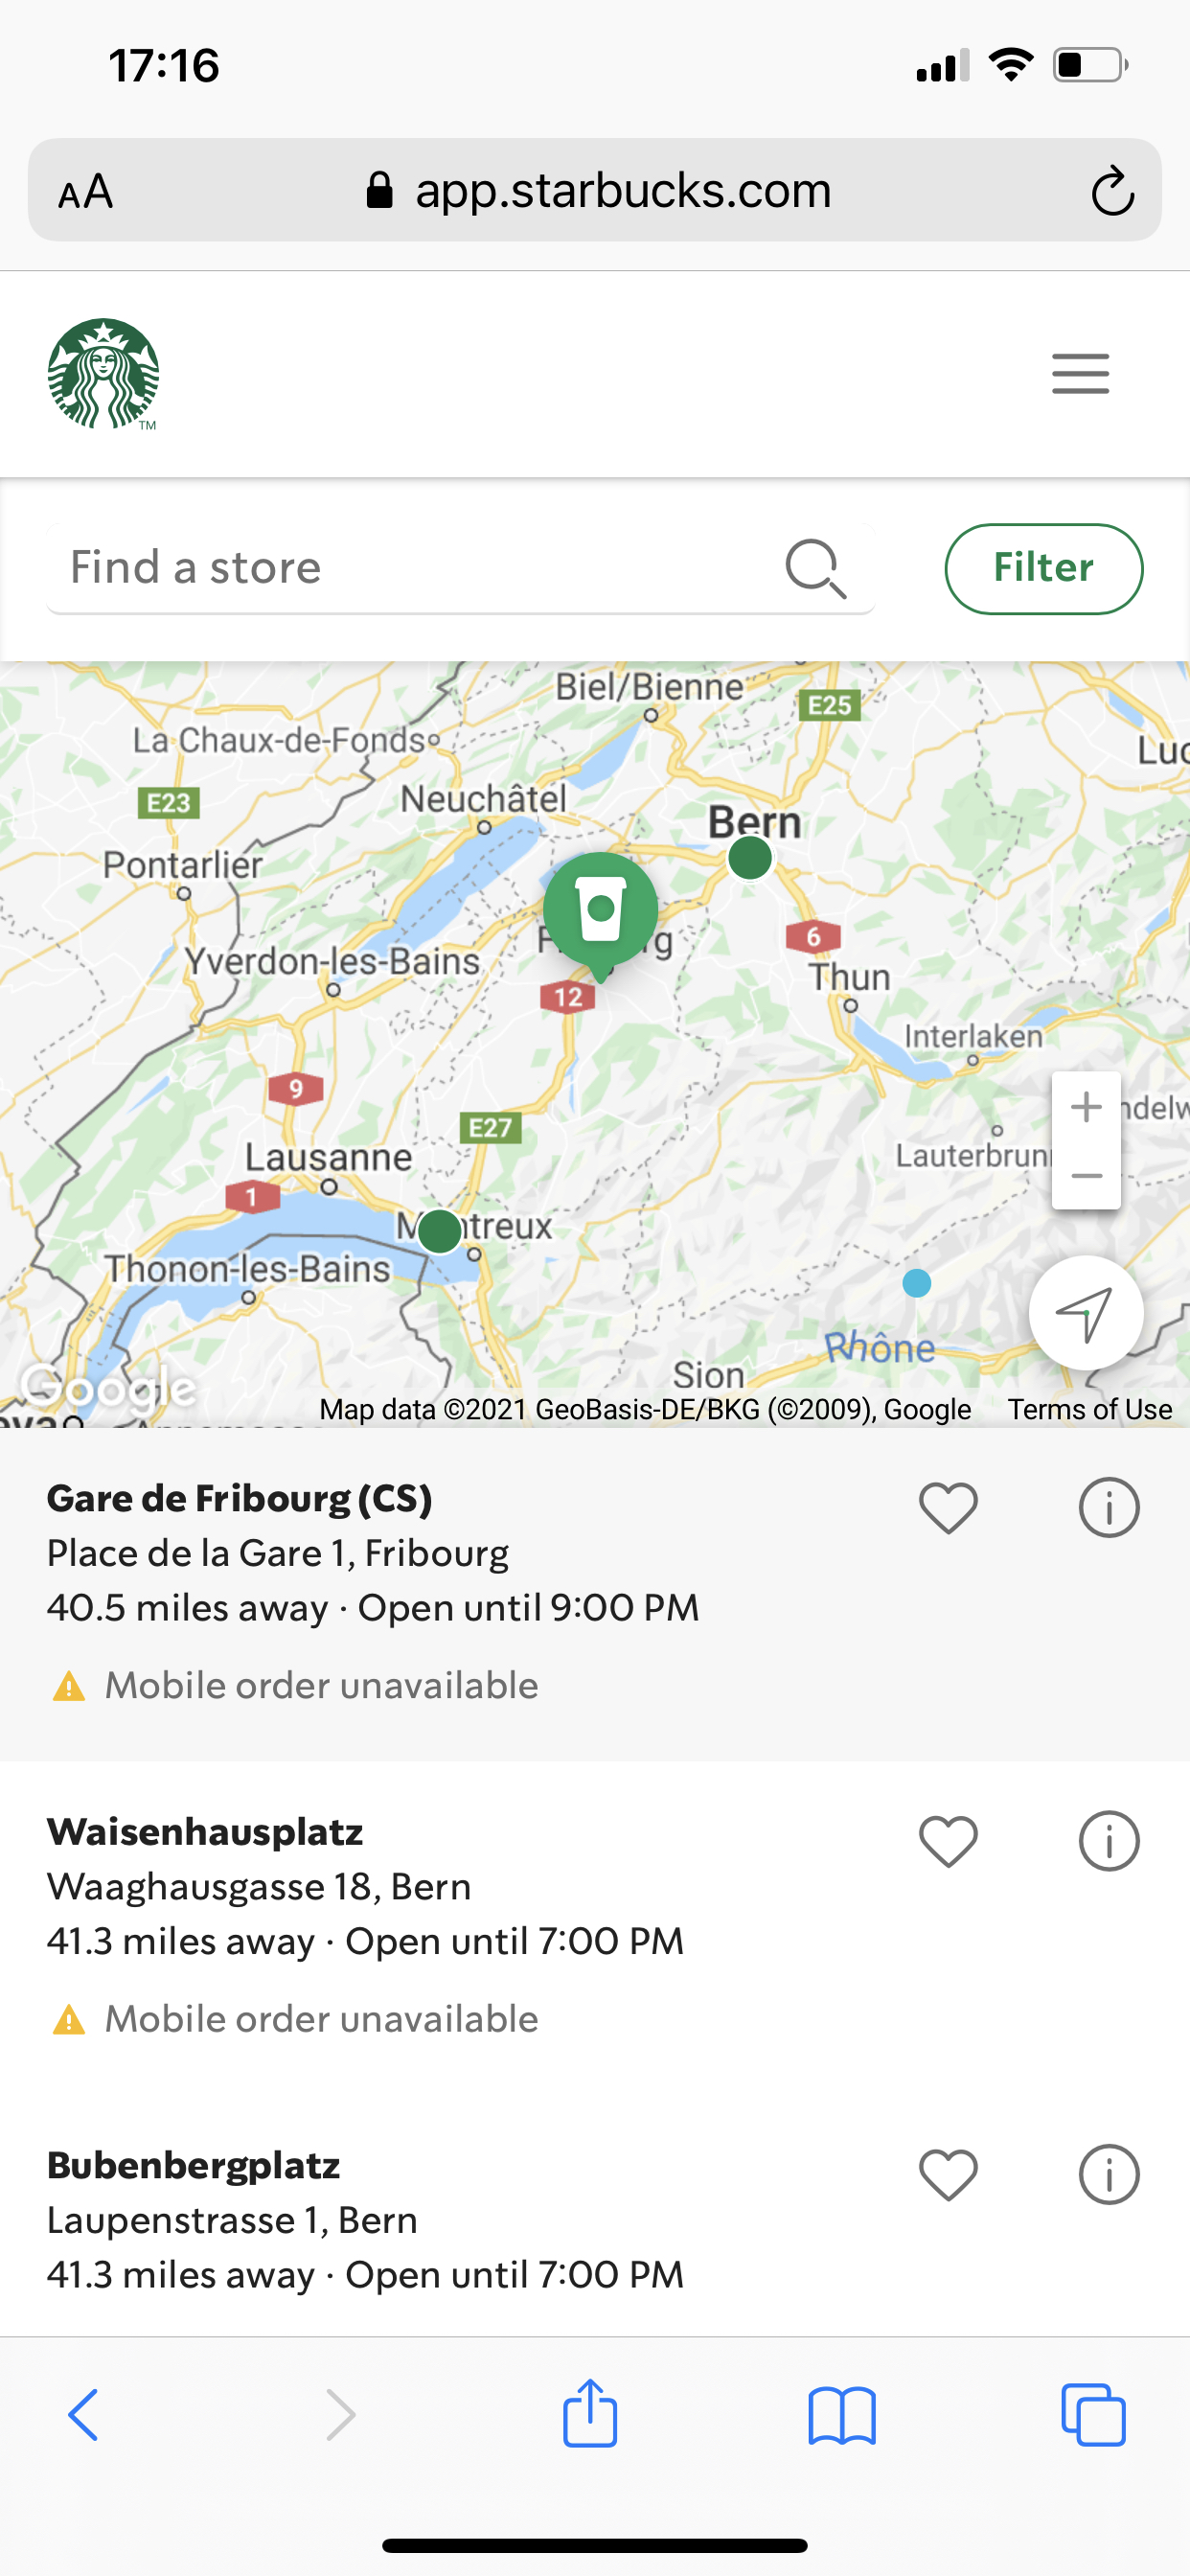
\includegraphics[scale=0.15]{images/starbucks_standort.jpeg}
	\caption[Standort in der Starbucks \ac{PWA}]{Standort in der Starbucks\ac {PWA},\\ Quelle: \cite{starbucksPwaStandort}}
	\label{img: Standort in der Starbucks PWA}
\end{figure}

\subsubsection{Fazit}
Die Applikation von Starbucks zeigt auf, was eine \ac{PWA} leisten kann. Sie dient als Vorbild für die Applikation der JTI-Pick-Up Station. 


\subsection{Fazit}
Es existieren diverse Produkte, welche einen ähnlichen Ansatz verfolgen wie dieses Projekt. Besonders hervorzuheben ist dabei die avec box. \ref{avecBox} Der Betreiber verfolgt hier einen ähnlichen Ansatz. 
Der Kaufvorgang bei Tabakwaren unterscheidet sich dabei kaum von dem in diesem Projekt umzusetzenden. Durch die Analyse des dort verwendeten Vorgehens konnte ein guter Überblick gewonnen werden. Zudem konnte auch gesehen werden, wie die Integration der Altersverifikation umgesetzt wurde. Dieses Wissen ist für die spätere, eigene Umsetzung sehr wichtig. \\
Die Applikation von Starbucks liefert einen sehr guten Überblick über die Möglichkeiten von \ac{PWA}'s. Besonders Designtechnisch ist diese Anwendung sehr wertvoll.\\
Die anderen analysierten Angebote lieferten keinen Mehrwert für das Projekt, da sie die gestellte Problematik nur bedingt oder gar nicht lösen.  

\newpage 